
\subsection{Long-Range Spatio-Temporal Task} \label{synth-benchmark:long}
Finally, to evaluate the ability of TGL methods to reason over both temporal and spatial dependencies, we introduce  \emph{long-range spatio-temporal tasks}. These tasks combine time delays with structural patterns, extending the delayed cause-and-effect setup to include long spatial paths.  At each time step, the graph contains paths originating from a source node \(v_{\mathcal S}\), while the target node \(v_{\mathcal T}\) connects to the endpoints of the paths generated $\lag$ time steps before.
 The task is formalized as follows:


\begin{definition}[Long-Range Spatio-Temporal Task]
\looseness-1 Let \(\lag, d, P \in \mathbb{N}\). The \emph{long-range spatio-temporal task} family $ \mathcal{L}\hspace{-0.035cm}\mathcal{R}_P(\lag,d)$ is defined over dynamic graphs \(\mathcal{G} = G_1, G_2, \dots\), where each snapshot $G_t = (V, E_t)$ has a fixed node set $V = \{v_{\mathcal S}, v_{\mathcal T}, v_1, \dots, v_{N}\}$. The edge set $E_t$ consists of $P$ disjoint paths of length $d$ from the source node $v_{\mathcal S}$ through randomly chosen intermediate nodes. For $t > \lag$, $E_t$ additionally includes $P$ edges from the target node $v_{\mathcal T}$ to the endpoints of the $P$ paths in $G_{t - \lag}$. Formally, for $t > \lag$:
$
E_t = \bigcup_{p=1}^P \{(v_{\mathcal S}, u_1^{(t,p)}), (u_1^{(t,p)}, u_2^{(t,p)}),\dots, (u_{d-1}^{(t,p)}, u_d^{(t,p)})\} \cup \{(v_{\mathcal T}, u_d^{(t-\lag,p)})\}$, where the nodes $u^{(t,p)}_{i}$ for $i=1,\dots,d$, $p=1,\dots,P$ are drawn at random in $\{v_1,\dots,v_N\}$~(without replacement).
\end{definition}\label{def:long_range}


Intuitively, we can treat node $v_\mathcal{S}$ as the \textit{progenitor} of some signal that 1) reaches a set of nodes that are spatially separated from $v_\mathcal{S}$ by a distance $d$ and 2) whose effect (connecting the nodes that it reached to node $v_\mathcal{T})$ is additionally delayed by $\lag$ timesteps.
An illustration of a dynamic graph for this task is given in Figure~\ref{fig:longrange}.
%Here, given $P = 3, d = 3$, observe that at $t = 1$, $S$ is connected to 3 paths of length 3. The terminal nodes of these paths, namely $8, 9, 11$ are then connected to target $T$ after a lag of 1. 
We will focus on the effect of the lag $\lag$  and distance $d$ in our experiments and set the number of path $P$ to $3$ in all tasks, which we will simply denote by $\longrange{\lag,d}$.

\begin{figure}
    \centering
    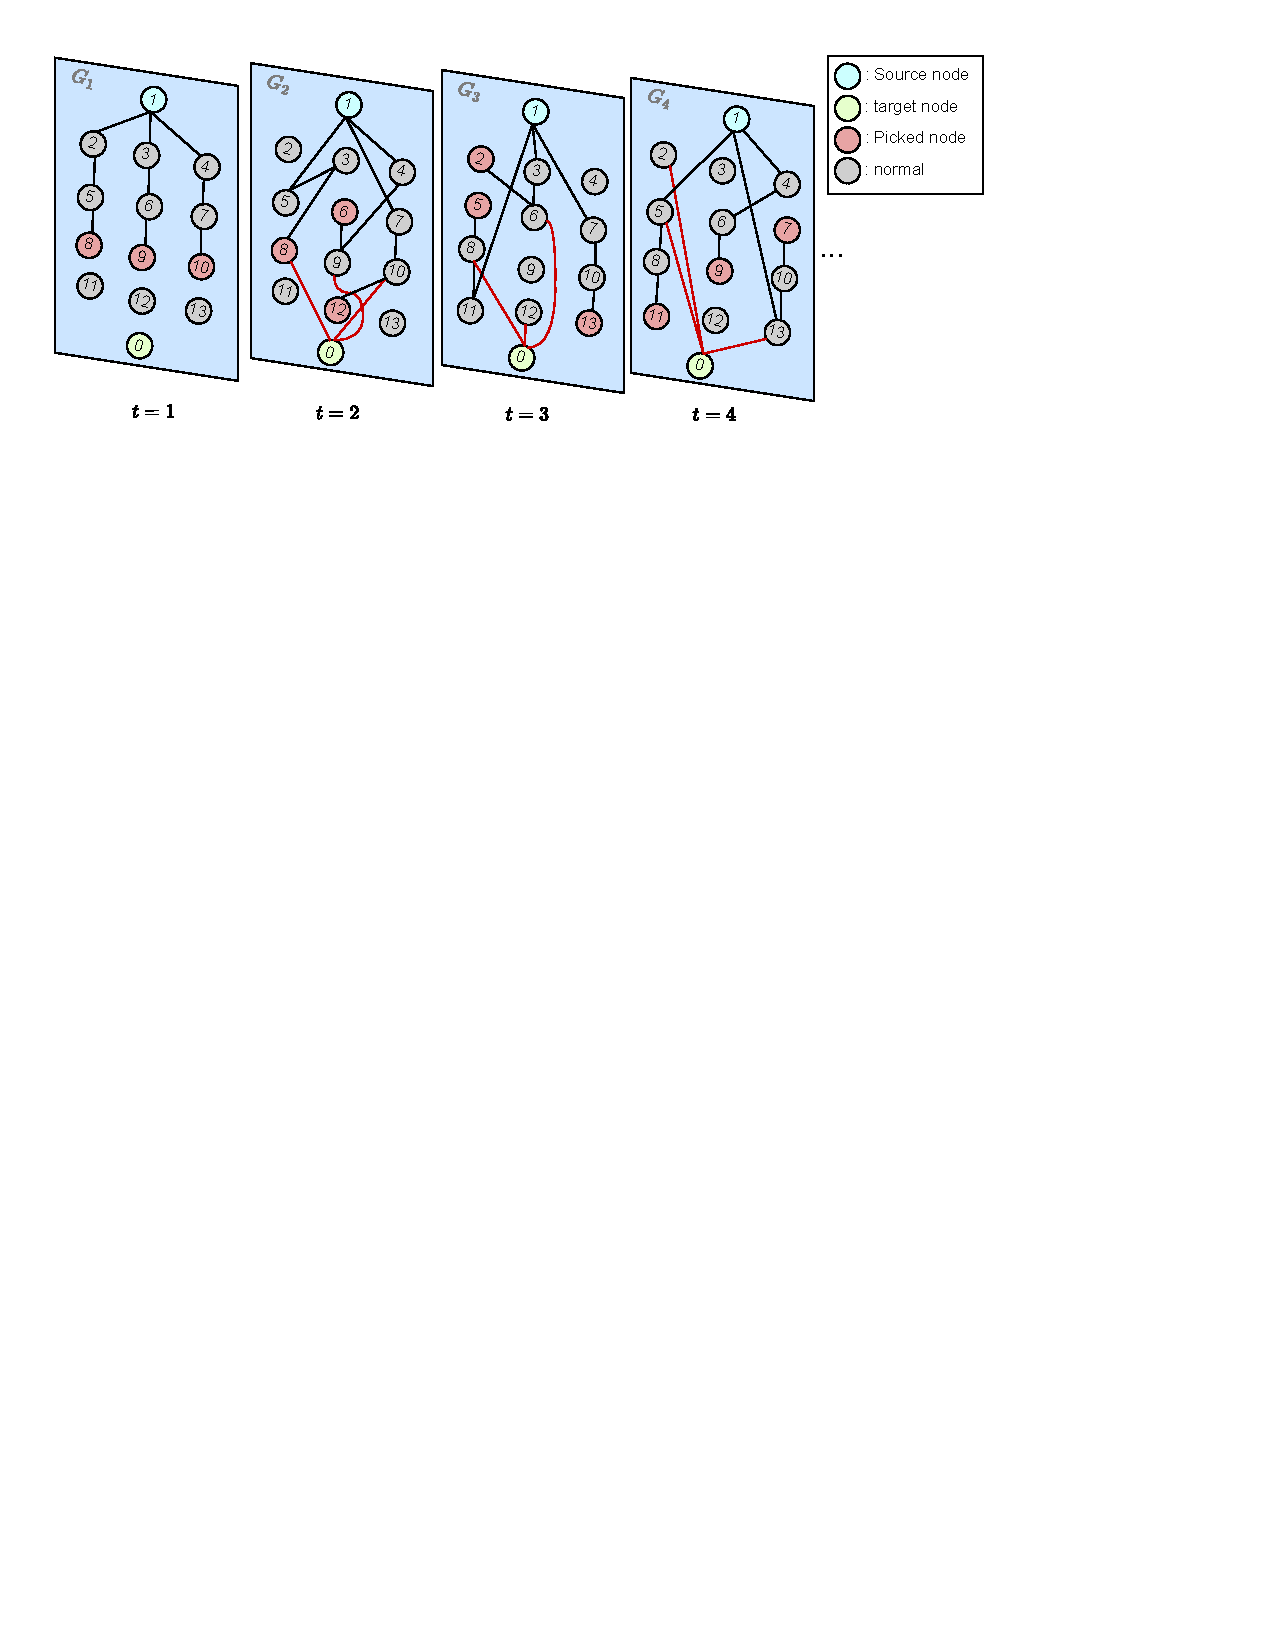
\includegraphics[width=0.8\linewidth, height=11.0em, keepaspectratio]{figs/long_range/fig.pdf}
    \caption{Illustration of a long-range spatio-temporal task $\longrange{\lag,d}$ with    $\ell=1$, $d=3$ and $P=3$.}
    \label{fig:longrange}
\end{figure}

\looseness-1 \textbf{Task objectives and datasets.}
In dynamic graphs, there are two natural notions of distances: distance between time steps and distance between nodes~(e.g., shortest path). Robust and powerful TGL methods should be able to reason and identify patterns simultaneously across these two dimensions. Tasks in \(\longrange{\lag,d}\) challenge TGL methods to jointly reason over long-term temporal dependencies and multi-hop spatial paths. The lag \(\lag\) determines how long information must be retained, while the distance \(d\) controls how far it must be propagated through the graph structure. This dual complexity makes the task a powerful benchmark for assessing the depth of spatio-temporal reasoning in TGL models.
To gradually increase the complexity of spatial and temporal dependencies, we generate tasks with distance values $d \in \{1, 2, 4, 8, 16\}$ and temporal lags $\lag \in \{1, 4, 16, 32\}$. 
%For each $(\ell, d)$ pair, we sample $4000+\lag$ timesteps, ensuring the effect subgraph appears in the final 4000 steps. As in the cause-and-effect task, the dynamic graph $G$ is divided into $80/10/10\%$ train/val/test splits. The number of paths is set to $P=3$ and we use $N=100$ intermediary nodes. 
% We fix $P=3$, and $n=12$, vary spatial distance $d \in \{1,2,4,8,16\}$ and temporal lag $l \in \{1,4, 16, 32\}$. For each $(l, d)$ we generate $2048$ timestep and split them $80/10/10\%$ (preserving entire lagged patterns), and report the average test $f_1$  score on the edge linking the target node $T$ to the endpoints of the $P$ path.
% In this section, we assess each of out selected method's ability to jointly reason over both spatial and temporal distances using the Long-Range Spatial-Temporal task (definition \ref{def:long_range}). 



\looseness-1 \textbf{Results.} Figure~\ref{fig:plots_long_range} shows $F_1$ scores for top-performing methods and the Edgebank baseline % (full results in the appendix~\ref{apendix:spatio_temporal_full_methods})
. When $\lag$ is small, DTDG models and DyGFormer perform well. However, as $\lag$ increases, DTDG performance drops sharply, exposing RNNs' limitations in long-range memory. DyGFormer degrades more gradually, but still struggles with extended dependencies. In contrast, TGAT and TGN remain robust at high lags ($\lag=16,32$), again highlighting the strength of attention-based message passing for this task. Yet, all models degrade as spatial distance exceeds $d=8$, underscoring the challenge of capturing long-range spatial dependencies even for the strongest temporal models.

% Figure~\ref{fig:plots_long_range} shows the $F_1$ scores among the best ranked methods~(results for all methods can be found in the appendix)  and the Edgebank baseline. When the $\lag$ is small, both DTDG methods and DyGFormer achieve strong performance. However, as $\ell$ increases, DTDG models's performance sharply drops, reflecting the limitations of RNN-based architectures to retain long-range temporal information. DyGFormer, though initially robust, also declines progressively with increasing lag, highlighting the challenge of modeling extended spatio-temporal dependencies without sufficient global context. In contrast, TGN and TGAT remain consistently resilient at higher lags ($\ell=16, 32$), outperforming others and showcasing the advantage of attention-based message-passing frameworks in maintaining long-term relational information. Nevertheless, as spatial distance grows, particularly beyond $d=8$, all methods experience noticeable degradation, suggesting the inherent difficulty of capturing spatial dependencies over extended paths, even for the strongest temporal models.


% \begin{figure}[H]
\begin{figure}[t]
    % (k, 1) CTDG
    \centering
    \begin{subfigure}[b]{0.24\textwidth}
        \centering
        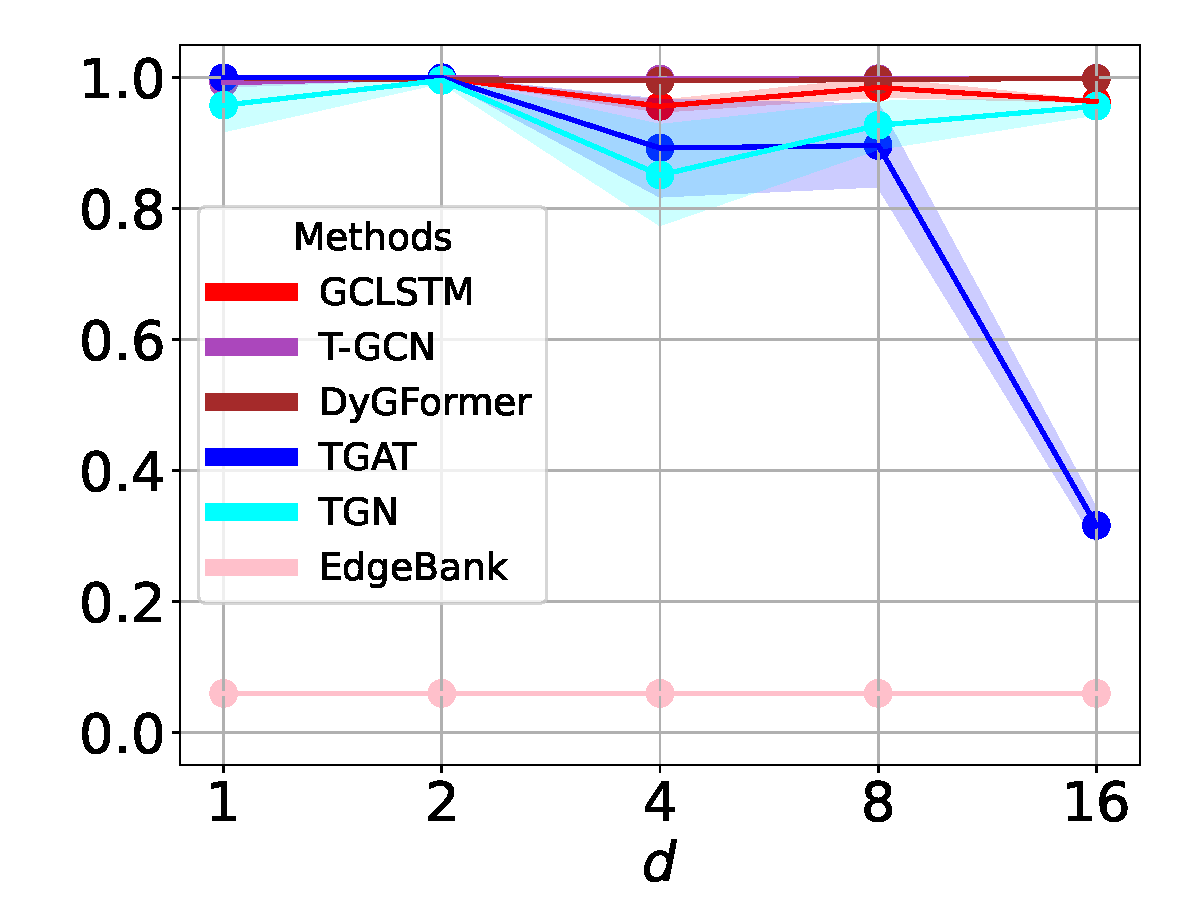
\includegraphics[width=\linewidth]{figs/long_range/fig(10, 10)/(1, d)Best_Test $F_1$.pdf}
        \caption{$(\ell=1, d)$}
        \label{fig:sub_long_range_(1,d)}
    \end{subfigure}
    \begin{subfigure}[b]{0.24\textwidth}
        \centering
        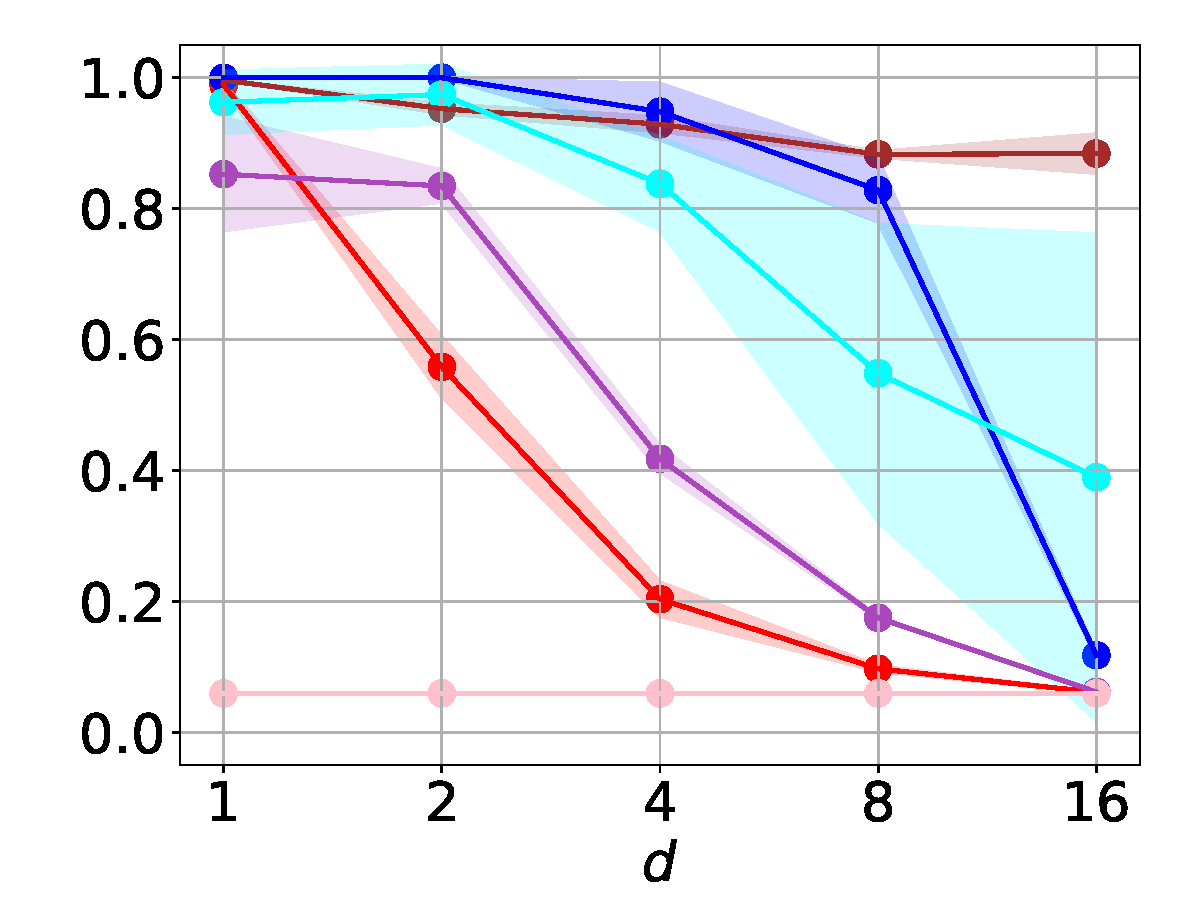
\includegraphics[width=\linewidth]{figs/long_range/fig(10, 10)/(4, d)Best_Test $F_1$.pdf}
        \caption{$(\ell=4, d)$}
        \label{fig:sub_long_range_(4,d)}
    \end{subfigure}
    %(k, 1) DTDG
    \centering
    \begin{subfigure}[b]{0.24\textwidth}
        \centering
        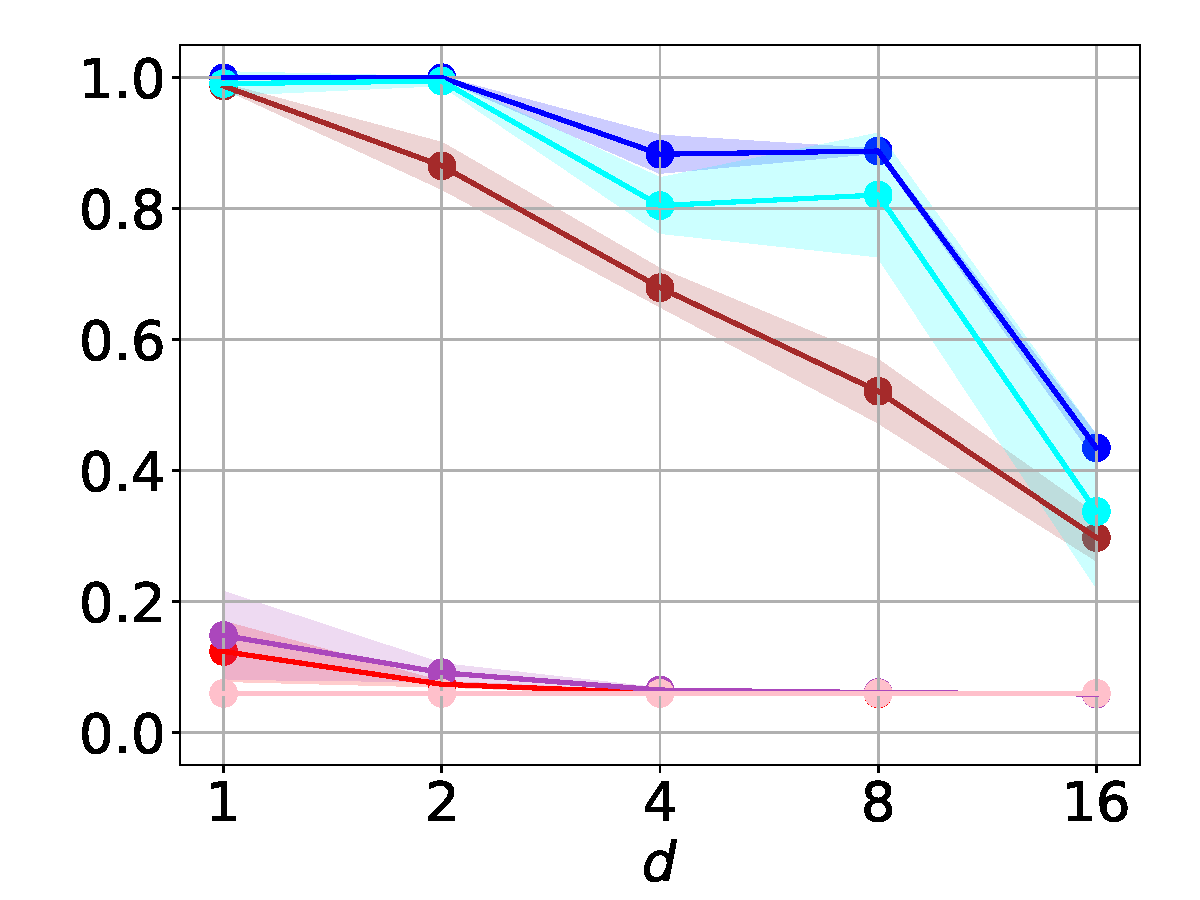
\includegraphics[width=\linewidth]{figs/long_range/fig(10, 10)/(16, d)Best_Test $F_1$.pdf}
        \caption{$(\ell=16, d)$}
        \label{fig:sub_long_range_(16,d)}
    \end{subfigure}
    \begin{subfigure}[b]{0.24\textwidth}
        \centering
        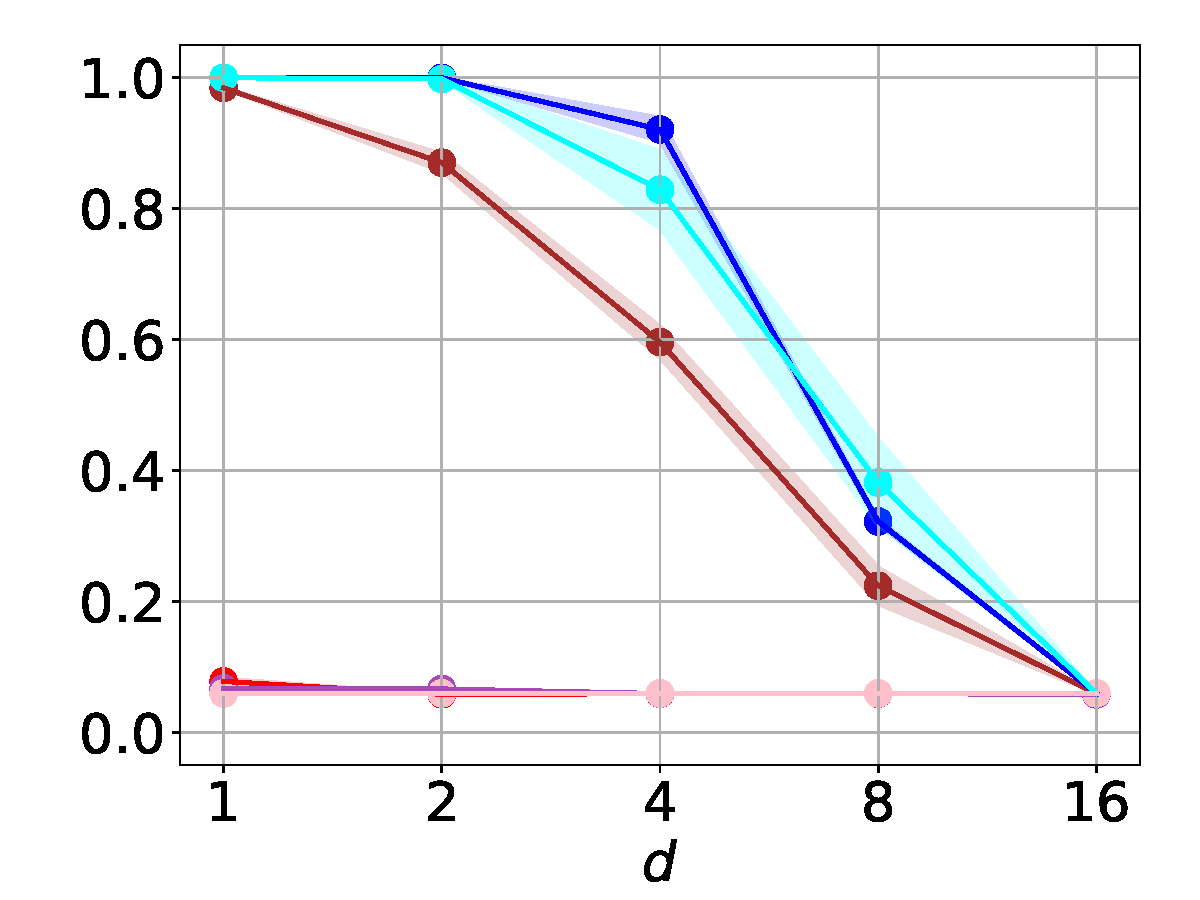
\includegraphics[width=\linewidth]{figs/long_range/fig(10, 10)/(32, d)Best_Test $F_1$.pdf}
        \caption{$(\ell=32, d)$}
        \label{fig:sub_long_range_(32,d)}
    \end{subfigure}
    
    \caption{Performance varying spatial and temporal distances in the long-range spatio-temporal tasks.}
    \label{fig:plots_long_range}
\end{figure}

% \begin{observation}[Long range ]
% DyGFormer is the best for small values of $\lag$ but gets worse when $\lag \geq 16$, wich can be explained by the limited context width: as $\lag$ gets bigger, some historical information gets out of the context 

% Surprising result for CTAN \ad{there is no CTAN here on the plots.}

% Message passing methods (TGN, TGAT) are quite good and robust to increasing values of the lag. 
% \end{observation}

